\documentclass{beamer}
\usepackage[english,russian]{babel}   % руссификации AmSLaTeX
\usetheme{CambridgeUS}

\usepackage{amsmath,amsfonts,amssymb,euscript,graphicx,wrapfig,multirow,mathtools,amsthm}
\usepackage{dsfont}

%%% Работа с картинками
\usepackage{graphicx}  % Для вставки рисунков
\graphicspath{{./images/}}  % папки с картинками
\setlength\fboxsep{3pt} % Отступ рамки \fbox{} от рисунка
\setlength\fboxrule{1pt} % Толщина линий рамки \fbox{}
\usepackage{wrapfig} % Обтекание рисунков и таблиц текстом
\usepackage[export]{adjustbox}
\usepackage{caption}
\usepackage{subcaption}
\usepackage{float}
\usepackage{tikz-cd}
\usetikzlibrary{babel}
\usepackage{animate}
\usepackage{tabularx}

%Algorithms
%http://blog.harrix.org/article/648
\usepackage[ruled,vlined]{algorithm2e}

\SetKwInput{KwData}{Исходные параметры}
\SetKwInput{KwResult}{Результат}
\SetKwInput{KwIn}{Входные данные}
\SetKwInput{KwOut}{Выходные данные}
\SetKwIF{If}{ElseIf}{Else}{если}{тогда}{иначе если}{иначе}{конец условия}
\SetKwFor{While}{до тех пор, пока}{выполнять}{конец цикла}
\SetKw{KwTo}{от}
\SetKw{KwRet}{возвратить}
\SetKw{Return}{возвратить}
\SetKwBlock{Begin}{начало блока}{конец блока}
\SetKwSwitch{Switch}{Case}{Other}{Проверить значение}{и выполнить}{вариант}{в противном случае}{конец варианта}{конец проверки значений}
\SetKwFor{For}{цикл}{выполнять}{конец цикла}
\SetKwFor{ForEach}{для каждого}{выполнять}{конец цикла}
\SetKwRepeat{Repeat}{повторять}{до тех пор, пока}
\SetAlgorithmName{Алгоритм}{алгоритм}{Список алгоритмов}

\DeclareMathOperator{\im}{im}
\DeclarePairedDelimiter\norm{\lVert}{\rVert}%
\newcommand{\quotient}[2]{{\raisebox{.2em}{$#1$}\left/\raisebox{-.2em}{$#2$}\right.}}

\makeatother
\setbeamertemplate{footline}
{
	\leavevmode%
	\hbox{%
		\begin{beamercolorbox}[wd=.8\paperwidth,ht=2.25ex,dp=1ex,center]{title in head/foot}%
			\usebeamerfont{title in head/foot}\insertshorttitle
		\end{beamercolorbox}%
		\begin{beamercolorbox}[wd=.2\paperwidth,ht=2.25ex,dp=1ex,center]{date in head/foot}%
			\insertframenumber{} / \inserttotalframenumber\hspace*{1ex}
	\end{beamercolorbox}}%
	\vskip0pt%
}
\makeatletter

\title{Применение персистентных гомологий для задачи классификации изображений}

\author{\small Обучающийся \qquad\qquad\qquad\qquad\qquad Снопов П.М.\\
		\enspace Руководитель \qquad  д.т.н., проф. \qquad Леденева Т.М.}
\institute[ВГУ]{{ Воронежский Государственный Университет} \\ 
				Факультет прикладной математики, информатики и механики \\[1em]
				Кафедра вычислительной математики и прикладных \\
				информационных технологий}

\date{\footnotesize Бакалаврская работа \\
	  Направление 01.03.02 Прикладная математика и информатика \\
  	  Профиль Математическое моделирование и вычислительная математика}


\begin{document}
	\begin{frame}[plain]
		\centering
		
		\begin{beamercolorbox}[sep=8pt,center,colsep=-4bp,rounded=true,shadow=true]{institute}
			\usebeamerfont{institute}\insertinstitute
		\end{beamercolorbox}
		
		{\usebeamercolor[fg]{titlegraphic}\inserttitlegraphic\par}
		
		\begin{beamercolorbox}[sep=8pt,center,colsep=-4bp,rounded=true,shadow=true]{title}
			\usebeamerfont{title}\inserttitle\par%
			\ifx\insertsubtitle\@empty%
			\else%
			\vskip0.25em%
			{\usebeamerfont{subtitle}\usebeamercolor[fg]{subtitle}\insertsubtitle\par}%
			\fi%     
		\end{beamercolorbox}%
		
		\vskip1em\par
		
		\begin{beamercolorbox}[sep=8pt,center,colsep=-4bp,rounded=true,shadow=true]{date}
			\usebeamerfont{date}\insertdate
		\end{beamercolorbox}\vskip0.5em
		
		\begin{beamercolorbox}[sep=8pt,center,colsep=-4bp,rounded=true,shadow=true]{author}
			\usebeamerfont{author}\insertauthor
		\end{beamercolorbox}
		
	\end{frame}
	\footnotesize
	\section{Введение}
		\subsection{Содержание}	
		\begin{frame}
		\frametitle{Содержание}
		\tableofcontents
	\end{frame}
		\subsection{Цель и задачи работы}
		\begin{frame}
		\frametitle{Цель и задачи работы}
			\textbf{\small Цель:} Исследование подхода, основанного на топологическом анализе данных, для классификации изображений \\[1em]
			\textbf{\small Задачи:}
			\begin{itemize}
				\item Изучение теоретических и практических основ топологического анализа данных
				\item Анализ подходов классификации изображений
				\item Формирование алгоритма на основе персистентных гомологий
				\item Проведение вычислительного эксперимента, выявление области применимости, плюсов и минусов данного подхода
			\end{itemize}
		\end{frame}
		\subsection{Актуальность}	
		\begin{frame}
		\frametitle{Актуальность}
			\begin{itemize}
				\item Классификация изображений -- фундаментальная задача анализа данных, одно из основных направлений ее развития, которое в последнее время имеет очень интенсивное развитие, связанное с достижениями нейронных сетей.
				%\item Несмотря на успех нейронных сетей, они обладают некоторыми недостатками, поэтому имеет смысл искать другие подходы к данной задаче.
				%\item Топологический анализ данных (ТДА) -- новая область анализа данных, которая использует различные техники из алгебраической топологии -- может предложить новые инструменты, которые могут быть применимы к данной задаче.
				\item Основным инструментом ТДА являются персистентные гомологии, о которых можно думать как об адаптации понятия гомологии к облаку точек. С помощью такого инструмента можно выявлять топологические характеристики исследуемого объекта.
				\item Задача классификации по сути является задачей определения характеристических свойств, которым удовлетворяют объекты одного класса. Поэтому персистентные гомологии могут быть полезны в данной задаче, так как зачастую такие свойства имеют геометрическую природу.
			\end{itemize}
	\end{frame}

	\section{Теоретические сведения}
		\subsection{Симплициальные комплексы}
		\begin{frame}
			\frametitle{Симплициальные комплексы}
			
			\begin{definition}
				Симплициальный комплекс $K$ -- это множество симплексов, т.е. выпуклых оболочек набора $n+1$ точек $\in \mathbb{R}^p$, таких, что векторы $ x_1 - x_0, ..., x_n - x_0 $ линейно независимы, при этом
				\begin{itemize}
					\setlength{\itemsep}{-1mm}
					\item Для каждого симплекса из $K$ его грани тоже лежат в $K$,
					\item Пересечение любых двух симплексов $\sigma, \tau \in K$ либо пусто, либо является гранью и $\sigma$, и $\tau$.
				\end{itemize}
			\end{definition}
			\begin{figure}
				\centering
				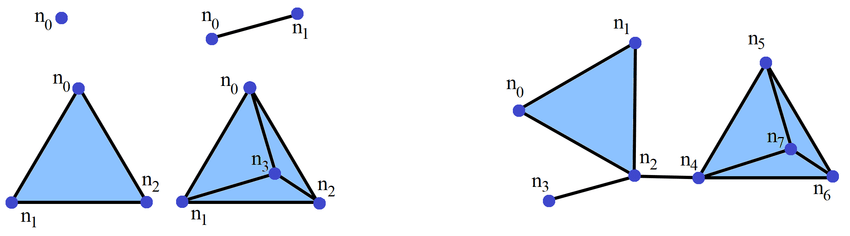
\includegraphics[width=\linewidth]{simplexAndComplex.png}
			\end{figure}
		\end{frame}
		\iffalse  %Rips complexes
		\begin{frame}
			\frametitle{Симплициальные комплексы}
			
			Имея облако точек $X \subset \mathbb{R}^n$, можно построить симплициальный комплекс по нему.  Наиболее популярные -- симплициальные комплексы \text{\it Чеха} и \text{\it Вьеториса—Рипса}.
			\begin{figure}
				\centering
				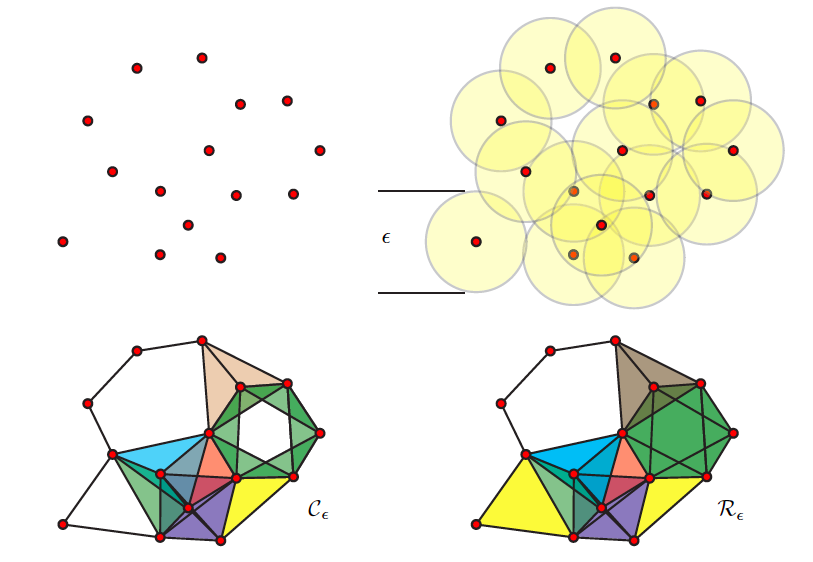
\includegraphics[scale=0.3]{complexes.png}
			\end{figure}
		\end{frame}
		\fi
		\subsection{Cимплициальные гомологии}
		\begin{frame}[fragile]
			\frametitle{Симплициальные гомологии}
			Рассмотрим свободную абелеву группу $C_k(K)$ $k\text{-цепей}$ симплициального комплекса $K$ и гомоморфизм $\partial_k : C_k(K) \to C_{k-1}(K)$ называют {\it граничным оператором}. Он удовлетворяет следующему свойству:
			\[
			\partial_{k-1} \circ \partial_k = 0.
			\]	
			Т.е. $ \im \partial_{k+1} \leq \ker \partial_k \leq C_k(K)$.
			
			Последовательность $C_k(K)$ и $\partial_k$ называется {\it цепным комплексом}
			
			\begin{center}
				\begin{tikzcd}[cells={nodes={minimum height=2em}}]
				... \arrow[r, "\partial_{k+2}"] & C_{k+1} \arrow[r,"\partial_{k+1}"]  &  C_k \arrow[r,"\partial_k"] &  C_{k-1} \arrow[r, "\partial_{k-1}"] & ... \arrow[r, "\partial_1"] & C_0.
				\end{tikzcd}
			\end{center}
		
			\begin{figure}[!htbp]
				\centering
				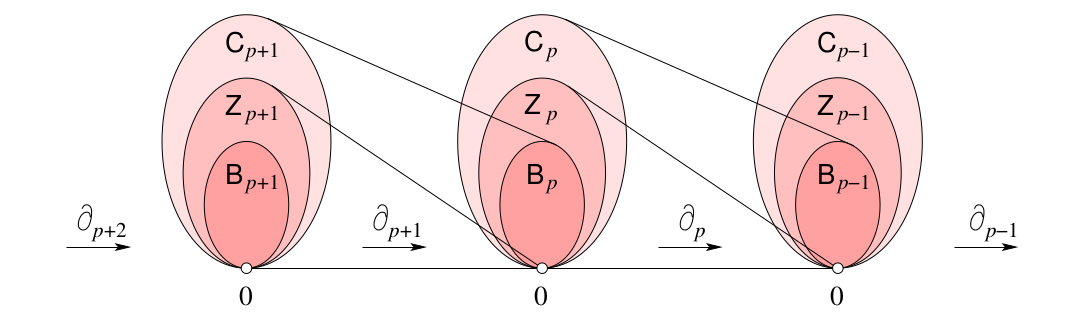
\includegraphics[width=0.5\linewidth, keepaspectratio=true]{chain.png}
				%\caption{Цепной комплекс}
				%\label{chain}
			\end{figure}
		\end{frame}
		\begin{frame}
			\frametitle{Симплициальные гомологии}
			\begin{definition}
				$k$-ой группой гомологий симплициального комплекса $K$ называют следующую фактор-группу:
				\[
				H_k(K) = \quotient{\ker \partial_k}{\im \partial_{k+1}}.
				\]
				
				Тогда $k$-ое число Бетти -- размерность $k$-ой группы гомологий: $\beta_k(K) = \dim H_k(K)$. 
			\end{definition}
			При $k=0$ число Бетти описывает количество компонент связности данного пространства. При $k=1$ -- количество циклов. При $k=2$ число Бетти описывает количество "полостей".
		\end{frame}
		\begin{frame}
			\frametitle{Симплициальные гомологии}
			\begin{center}
				\begin{table}[!htbp]
					\centering
					\begin{tabular}{ |c|c c c| }
						\hline
						Пространство & $\beta_0$ & $\beta_1$ & $\beta_2$ \\ 
						\hline
						Pt & 1 & 0 & 0 \\ 
						$D^2$ & 1 & 0 & 0 \\ 
						Треугольник & 1 & 0 & 0 \\
						Граница треугольника & 1 & 1 & 0 \\
						$S^1$ & 1 & 1 & 0 \\
						$S^2$ & 1 & 0 & 1 \\
						$\mathbb{T}^2 = S^1 \times S^1$ & 1 & 2 & 1 \\
						\hline
					\end{tabular}
					\caption{Первые числа Бетти для некоторых пространств}
				\end{table}
			\end{center}
		\end{frame}
		\subsection{Фильтрации и устойчивые гомологии}
		\begin{frame}
			\frametitle{Как построить симплициальный комплекс?}
			
			Имея облако точек $X \subset \mathbb{R}^n$, можно построить симплициальный комплекс по нему.  Наиболее популярные -- симплициальные комплексы \text{\it Чеха} и \text{\it Вьеториса—Рипса}.
			\begin{figure}
				\centering
				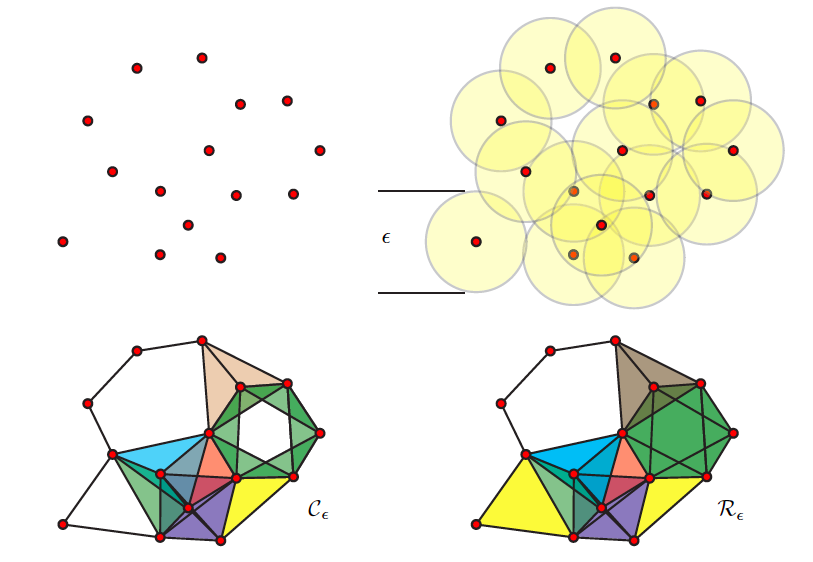
\includegraphics[scale=0.3]{complexes.png}
			\end{figure}
		\end{frame}
		\begin{frame}
			\frametitle{Фильтрации и устойчивые гомологии}
			{\it Фильтрацией симплициального комплекса $K$} называют вложенное семейство подкомплексов $ (K_\tau)_{\tau \in T} $, такое, что если $ \tau < \tau^{'} $, то $ K_\tau \subseteq K_{\tau^{'}} $.
			\begin{definition}
				$n$-ыми устойчивыми гомологиями фильтрованного комплекса $ (K_\tau)_{\tau \in T} $ называют проиндексированное семейство абелевых групп и гомоморфизмов между ними $H_n(T) = \{ (H_n(K_\tau))_{\tau \in T} $, $ (H_n(K_\tau) \to H_n(K_\tau^{'}))_{\tau \leq \tau^{'}} \}$.
			\end{definition}
			\begin{figure}
				\centering
				
\includegraphics[width=\linewidth]{filtration.png}
			\end{figure}
		\end{frame}
		\begin{frame}%[fragile]
			\frametitle{Фильтрации и устойчивые гомологии}
			Устойчивые гомологии -- это пример конечнопорожденного персистентного модуля. 
			Главная теорема для конечнопорожденного персистентного модуля -- это структурная теорема:
			\begin{theorem}[Структурная теорема для конечнопорожденного персистентного модуля]
				Пусть $R$ -- произвольное поле, а $(A_*, x)$ -- конечнопорожденный персистентный $R$-модуль. Тогда $(A_*, x)$ имеет единственное с точностью до перестановки слагаемых представление в виде прямой суммы конечного числа интервальный модулей:
				\[
				(A_*, x) \simeq \big( \bigoplus\limits_{k} I_{[j_k, s_k]} \big) 
				\oplus 
				\big( \bigoplus\limits_{k} I_{[r_k, \infty)} \big)
				\]
			\end{theorem}
		\end{frame}	
		\begin{frame}
			\frametitle{Фильтрации и устойчивые гомологии}
			\begin{figure}
				\centering
				\begin{subfigure}{.45\textwidth}
					\centering
					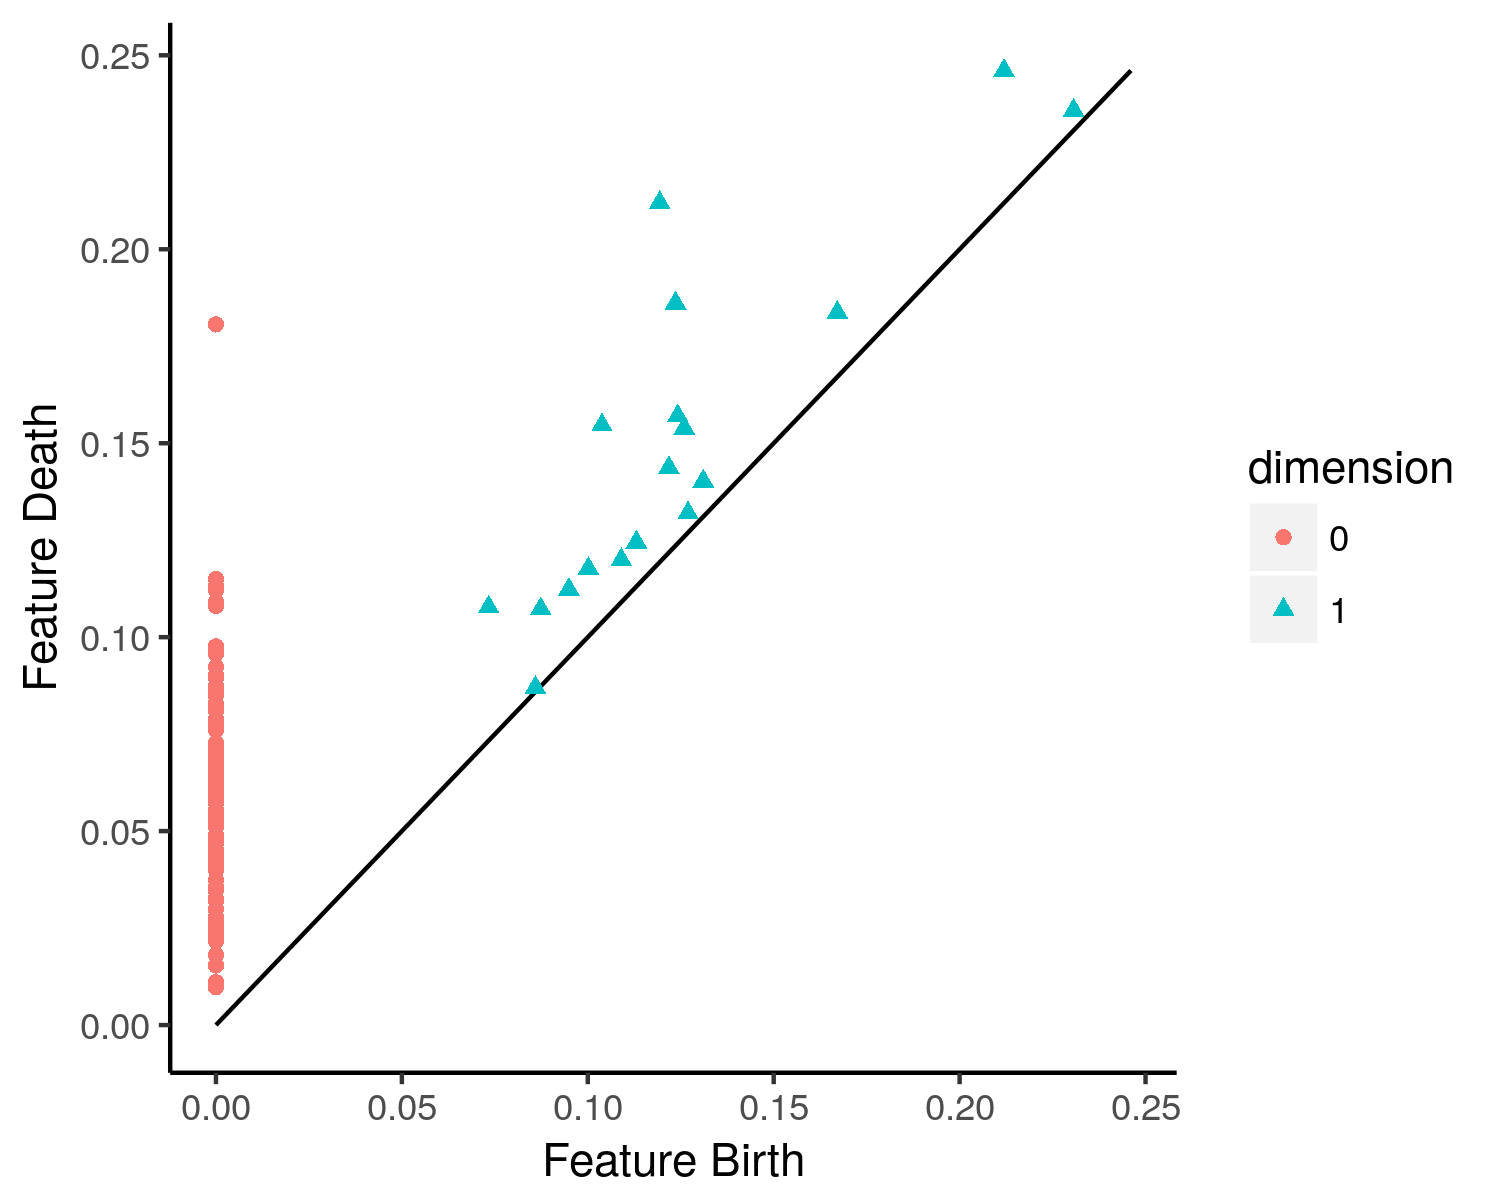
\includegraphics[scale=0.5, width=\linewidth]{persist_diag.png}
					\caption{Диаграмма персистентности}
				\end{subfigure}
				\begin{subfigure}{.45\textwidth}
					\centering
					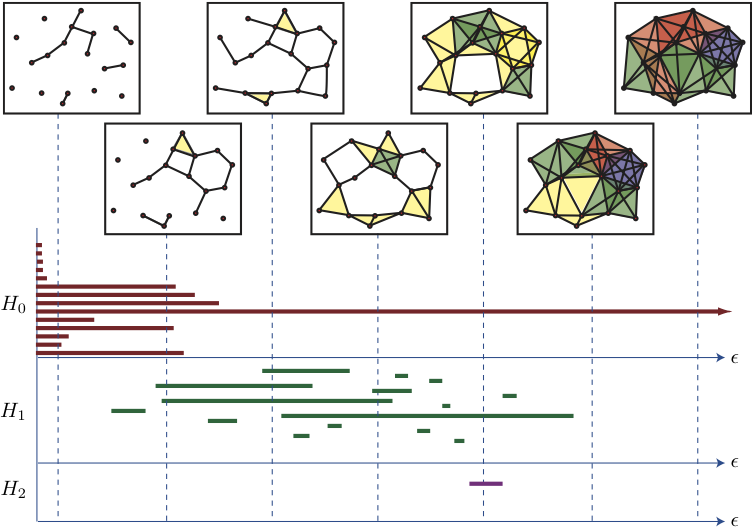
\includegraphics[width=\linewidth]{barcode.png}
					\caption{Баркод}
				\end{subfigure}
				\caption{Способы кодирования информации об персистентных гомологиях}
			\end{figure}
		\end{frame}
		\subsection{Векторизация диаграмм персистентности}
		\begin{frame}
			\frametitle{Метрическое пространство всех диаграмм персистентности}
			На множестве $\mathcal{D}$ диаграмм персистентности можно ввести структуру метрического пространства. Например, можно ввести т.н. {\it $p-$метрику Васерштейна} $W_p$, где $1 \leq p < \infty$:
			\[
			W_p(B,B^{'}) = \inf\limits_{\gamma:B\to B^{'}} 
			\big( 
			\sum\limits_{u \in B} \norm{u - \gamma(u)}_\infty^p
			\big) ^{\frac{1}{p}},
			\]
			где $B, B^{'}$ -- диаграммы персистентности. 
			
			Другой естественной метрикой является т.н. {\it bottleneck distance} $W_\infty$:
			\[
				W_\infty(B, B^{'}) = \inf\limits_{\gamma:B\to B^{'}} \sup\limits_{u \in B}
										\norm{u - \gamma(u)}_\infty
			\]
		\end{frame}
		\begin{frame}
			\frametitle{Векторизация диаграмм персистентности}
			{\it Векторизацией для пространства диаграмм персистентности} называют отображение $ \varphi: \mathcal{D} \to V $, где $V$ -- векторное пространство. 
			
			{\it Амплитудой} на $\mathcal{D}$ называют отображение $A: \mathcal{D} \to \mathbb{R}$, для которого $\exists \varphi: \mathcal{D} \to V$, где $V$ -- нормированное пространство, такое, что $ \forall B \in \mathcal{D}: \;\; A(B) = \norm{\varphi(B)}$.
			
			{\it Персистентной энтропией} $E(B)$ диаграммы $B = \{ (b_i, d_i) \}_{i \in I}$ называют меру энтропии по Шеннону точек на диаграмме персистентности:
			\[
				E(B) = - \sum\limits_{i \in I} p_i \log(p_i), \text{ где $p_i = \dfrac{d_i - b_i}{\sum\limits_{i \in I}d_i-b_i}$. }
			\]
		\end{frame}
	
	\section{Алгоритм классификации}
		\subsection{Алгоритм построения векторного представления}
		\begin{frame}
			\frametitle{Общая идея алгоритма}
			\begin{itemize}
				\item По изображению строим фильтрацию;
				\item По построенной фильтрации находим кубический комплекс, персистентные гомологии и строим диаграмму устойчивости;
				\item Векторизуем диаграмму устойчивости, получаем векторное представление, которое можно использовать в моделях машинного обучения.
			\end{itemize}
		\end{frame}
		\begin{frame}
			\frametitle{Пайплайн используемого метода построения векторного представления}
			Построить фильтрацию для изображения можно различными методами. В настоящей работе было построено 17 разнообразных фильтрацией, для каждой из которых были получены $0$ и $1$ персистентные гомологии, из диаграмм которых было получено 14 признаков. Таким образом, для одной картинки было получено $17 \times 2 \times 14 = 476$ признаков.
			\begin{figure}
				\centering
				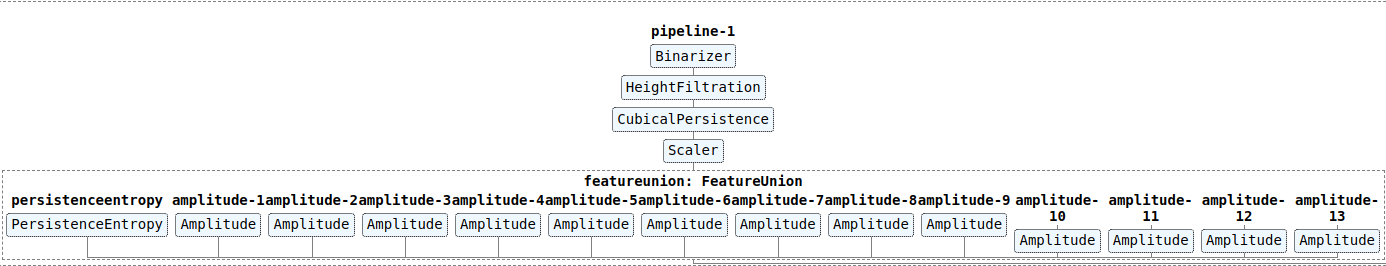
\includegraphics[width=\linewidth]{pipelineDiagram.png}
			\end{figure}
		\end{frame}
		\begin{frame}
			\frametitle{Процесс получения векторного представления}
			\begin{figure}
				\centering
				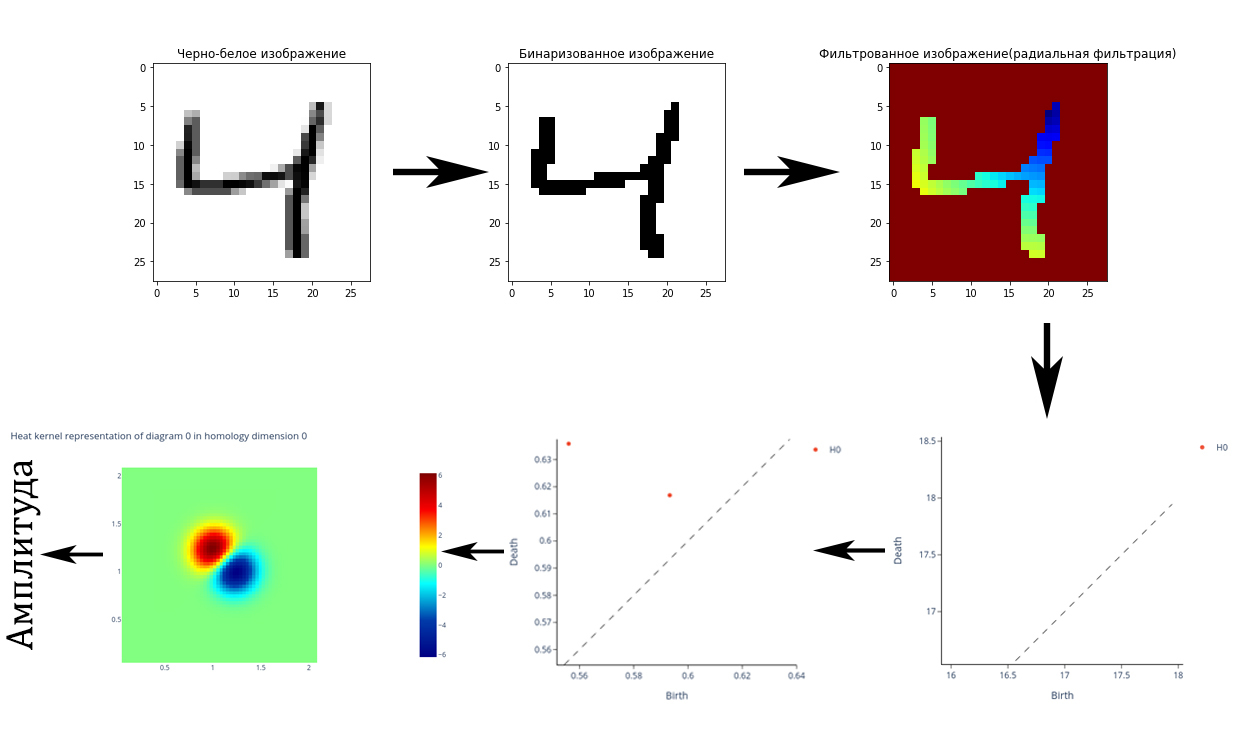
\includegraphics[width=\linewidth]{pipe.jpg}
			\end{figure}
		\end{frame}
		\subsection{Полученные результаты}
		\begin{frame}
			\frametitle{Сравнение результатов различных методов машинного обучения}
			\begin{center}
				\begin{table}[!htbp]
					\centering
					\begin{tabular}{ |c|c| }
						\hline
						Модель & Точность на тестовой выборке \\ 
						\hline
						Случайный лес & $0.88$  \\ 
						Логистическая регрессия & $0.9$ \\ 
						Метод опорных векторов & $0.88$  \\
						LightGBM & $0.86$ \\
						CatBoost & $0.88$ \\
						XGBoost & $0.88$  \\
						\hline
					\end{tabular}
					\caption{Сравнение результатов различных методов машинного обучения}
				\end{table}
			\end{center}
		\end{frame}
		\begin{frame}
			\frametitle{Сравнение результатов различных методов машинного обучения}
			\begin{center}
				\begin{table}[!htbp]
					\centering
					\begin{tabular}{ |c|c| }
						\hline
						Модель & Точность на тестовой выборке \\ 
						\hline
						Случайный лес & $0.88$  \\ 
						Логистическая регрессия & $0.9$ \\ 
						Метод опорных векторов & $0.9$  \\
						LightGBM & $0.88$ \\
						CatBoost & $0.89$ \\
						XGBoost & $0.89$  \\
						\hline
					\end{tabular}
					\caption{Сравнение результатов различных методов машинного обучения с подобранными гиперпараметрами}
				\end{table}
			\end{center}
		\end{frame}
		\begin{frame}
			\frametitle{Подбор гиперпараметров и отбор признаков}
			\begin{figure}[t]
				\centering
				\begin{subfigure}{.45\textwidth}
					\centering
					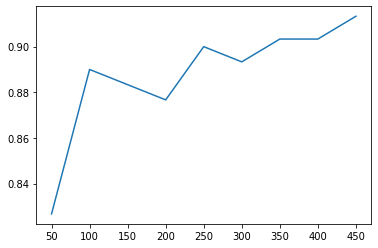
\includegraphics[scale=0.5, width=\linewidth]{accuraciesNumFeatures.png}
					\caption*{График зависимости точности на обучающей выборке и числа признаков}
				\end{subfigure}
				\begin{subfigure}{.45\textwidth}
					\centering
					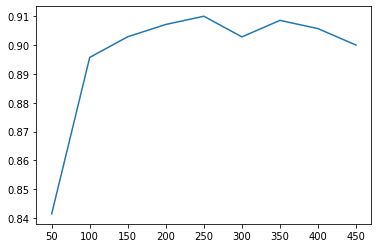
\includegraphics[width=\linewidth]{scoresNumFeatures.png}
					\caption*{График зависимости точности на валидационной выборке и числа признаков}
				\end{subfigure}
			\end{figure}
		\end{frame}
	
	\section{Заключение}
		\subsection{Что осталось сделать?}
		\begin{frame}
			\frametitle{Что осталось сделать?}
			\begin{itemize}
				\item Сравнить различные модели, которые обучались на топологических признаках, с теми же моделями, но которые обучаются прямо на картинке(т.е. в качестве признака берется каждый пиксель). Сравнить зависимости точности от количества признаков. Ожидаемый эффект: модели, обученные на топологических признаках, дают сравнимую точность при гораздо меньшем количестве признаков.
				\item Использовать топологический пайплайн как один из слоев нейросети, применить такую модель, сравнить результаты.
				\item Увеличить количество топологических признаков: использовать другие методы фильтрации и векторизации.
				\item Попробовать сделать отбор признаков на основе, например, коэффициента корреляции Пирсона. 
				\item Попробовать обучить модели на полном датасете. Вероятно тут нужно будет использовать батчи для создания векторного представления. Можно будет попробовать связанные с этим трюки в духе batch normalization.  
			\end{itemize}
		\end{frame}
		\subsection{Заключение}
		\begin{frame}
			\centering
			
			\begin{beamercolorbox}[sep=8pt,center,colsep=-4bp,rounded=true,shadow=true]{institute}
				\usebeamerfont{institute}\insertinstitute
			\end{beamercolorbox}
			
			{\usebeamercolor[fg]{titlegraphic}\inserttitlegraphic\par}
			
			\begin{beamercolorbox}[sep=8pt,center,colsep=-4bp,rounded=true,shadow=true]{title}
				\usebeamerfont{title}\inserttitle\par%
				\ifx\insertsubtitle\@empty%
				\else%
				\vskip0.25em%
				{\usebeamerfont{subtitle}\usebeamercolor[fg]{subtitle}\insertsubtitle\par}%
				\fi%     
			\end{beamercolorbox}%
			
			\vskip1em\par
			
			\begin{beamercolorbox}[sep=8pt,center,colsep=-4bp,rounded=true,shadow=true]{date}
				\usebeamerfont{date}\insertdate
			\end{beamercolorbox}\vskip0.5em
			
			\begin{beamercolorbox}[sep=8pt,center,colsep=-4bp,rounded=true,shadow=true]{author}
				\usebeamerfont{author}\insertauthor
			\end{beamercolorbox}
			
			
		\end{frame}
\end{document}